 %%%%%%%%%%%%%%%%%%%%%%%%%%%%%%%%%%%%%%%%%%%%%%%%%%%%%%%%%%%%%%%%%%%%%%%%%%%%%%%%%%
%%																				%%
%% File name: 		01sarah.tex													%%
%% Project name:	Hochleistungsantenne										%%
%% Type of work:	T3X00 project work											%%
%% Author:		Sarah Brückner, Maximilian Stiefel, Hannes Bohnengel		%%
%% Date:		27th Arpil 2016												%%
%% University:		DHBW Ravensburg Campus Friedrichshafen						%%
%% Comments:		Created in gedit with tab width = 4							%%
%%																				%%
%%%%%%%%%%%%%%%%%%%%%%%%%%%%%%%%%%%%%%%%%%%%%%%%%%%%%%%%%%%%%%%%%%%%%%%%%%%%%%%%%%

\chapter{Amateurfunksatelliten}
In dieser Studienarbeit soll die Bodenstation erdnahe Satelliten verfolgen können. Erdnah bedeutet auf einer niedrigen Umflaufbahn bis etwa 1200 km. 
Dazu gehören die Amateurfunksatelliten, welche der Satellitenkommunikation zwischen Funkamateuren und auch zu experimentellen Zwecken dienen. 
Diese kommunizieren im 2-Meter- und 70-Zentimeterband und ermöglichen einen internationalen Sprech- und Datenfunk. Außerdem senden diese Satelliten
auch Messwerte der Betriebsdaten des Satelliten. Diese Satelliten werden meist von Hochschulen oder Amateurfunkvereinigungen gebaut und mit weiteren 
Satellisten an Board einer Rakete in das All geschossen. Dabei handelt es sich um kleine, leichte Satelliten, auch ``'Cubesat''' genannt.
\begin{figure}[h]
 \centering
 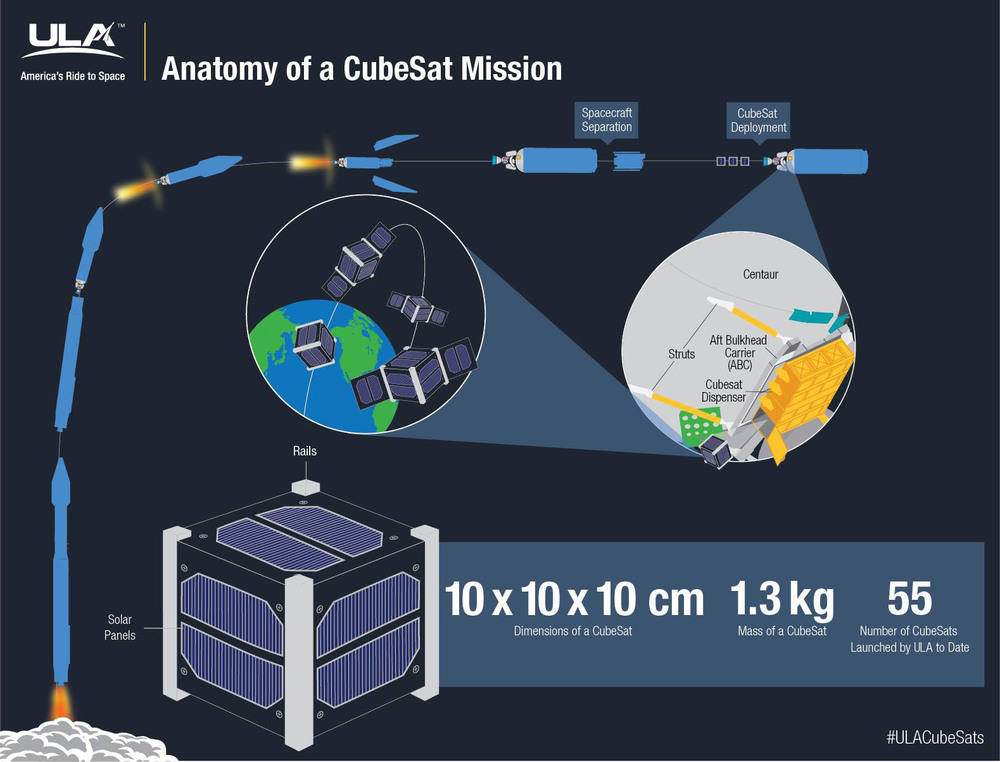
\includegraphics[width=0.8\linewidth]{./images/cubesat}
 \caption{Cubesat, Quelle: \cite{cubesat}}
 \label{fig:cubesat}
\end{figure}
Die Grafik zeigt einen beispielhaften Cubesat. Im Vergleich der ASTRA 1L Satellit mit einer Spannweite von 20 Meter und einem Gewicht von 4,5 Tonnen.

\newpar
